% change this if you want to work in english, or use a different bibliography
% style
%
% For instance, the following would use apa7:
% bibstyle=apa
%
% If your document is in English instead of Dutch, simply remove dutch
% (do not add 'english')
%
% Ex: \documentclass[bibstyle=apa]{adsai}
%
% would make an English document with an apa7-compliant bibliography
%
% Ex: \documentclass[bibstyle=ieee, dutch]{adsai}
%
% would make a Dutch document with an ieee-compliant bibliography
%
% you can mix and match these as you wish.
\documentclass{adsai}

% the title of your project
\title{PROJECT TITLE}
% the title of the module, such as 'Design Science Research' or 'Data Science'
\modulename{MODULE NAME}

% list of authors
\author{
student 1 (1234567890) \\
student 2 (1234567890) \\
student 3 (1234567890) \\
student 4 (1234567890) \\
name 1 (supervisor) \\
name 2 (supervisor)
}

% academic year that this document is due in
\academicyear{2025/2026}
% the period that this document is due in
\period{Q1}
% the date that this document is due
\date{01-01-2026}

\begin{document}
\maketitle % this adds the title, authors etc. to the beginning of your document

\newpage

\abstract{Maximum of 200 words: The abstract is a summary of the extended abstract as a whole. This implies that at least the following components from the extended abstract are included in summary form in the abstract: reason, objective, method, results and conclusion}

\thispagestyle{empty}

\newpage

\section{Introduction}

Maximum of 800 words (for background and goal combined)

\subsection{Background}
The background describes the context in which the assignment was carried out:
\begin{itemize}
    \item The companies/organizations involved and the products and/or services they provide
    \item The stakeholders, including the client
    \item The problem, need or opportunity that is the reason for the assignment
\end{itemize}

\subsection{Goal}
The goal logically follows from the background and describes the assignment to be carried out in a concise but concrete manner:
\begin{itemize}
    \item The goal to be achieved (for the client)
    \item Any further specification of that goal in the form of boundary conditions and/or requirements (if present)
    \item The specific artefact(s) to be delivered, if already known at the start of the work
\end{itemize}

\section{Theoretical Framework}

Maximum of 800 words. Not required for courses other than the Design Science Research minor. 

The theoretical framework describes the results of a (quick) literature scan with which the assignment to be carried out is classified on the basis of:
\begin{itemize}
    \item The problem, the opportunity or the need in the application domain,
    \item The (possible) solution(s)
    \item The innovative character 
\end{itemize}

The results of the literature scan show on the one hand to which category the problem belongs and on the other hand which (from existing work, i.e. broadly supported) uncertainties (with regard to the approach and/or end result) exist within the assignment.

\section{Methods}

Maximum of 1200 words. 

The method describes the entire approach, so that others can in principle reproduce the work. The description of the method takes place at 3 levels. 

First, the chosen overall method is described, in line with the objective of the assignment. Within the HBO-ICT program for example, assignments often consist of creating a (partly) innovative artifact (product or service). Design Science Research (DSR) is the standard method within the program for such design-oriented research. 

Subsequently, the concrete steps carried out within the chosen method are described in the form of phases and/or activities. It becomes clear whether these were carried out sequentially, parallel and/or iteratively. An illustration is highly recommended here. Specific from the DSR method should in any case be included: identifying requirements, carrying out grounding, designing, developing and testing the product or service and
disseminating the results of the work carried out. The field test from the DSR framework is optional, as a rule students will not arrive at a product that is ripe enough for a field test within the boundaries of the education.

Last but not least, the methods/methods used specifically within the phase(s) / activity(ies) are described concretely and in depth, where possible consisting of best or good practices. It is always important that the choices made are substantiated in relation to the context and objective of the assignment

\section{Results}

Maximum of 1200 words.

The results describe in depth the actual, substantive results achieved, logically
following from the method used. Name the concrete artefact that (for the client) forms the end product of the delivered work. Indicate what type of artefact it is, for example a design, an architecture, a model or a software application. Then describe in depth the content of the artefact based on the (which?) requirements, the (which?) relevant insights from grounding and the (which?) relevant insights from
activities within the design cycle. Use illustrations where useful, this is very clarifying compared to texts in (long) paragraphs only. Where possible, also use lists and/or tables for readability.

% Code below is an example of how various things in LaTeX can be inserted, such as code snippets, tables, etc.

\subsection{Examples}

Inserting an image can be done as followS:

\begin{figure}[H]
    \centering
    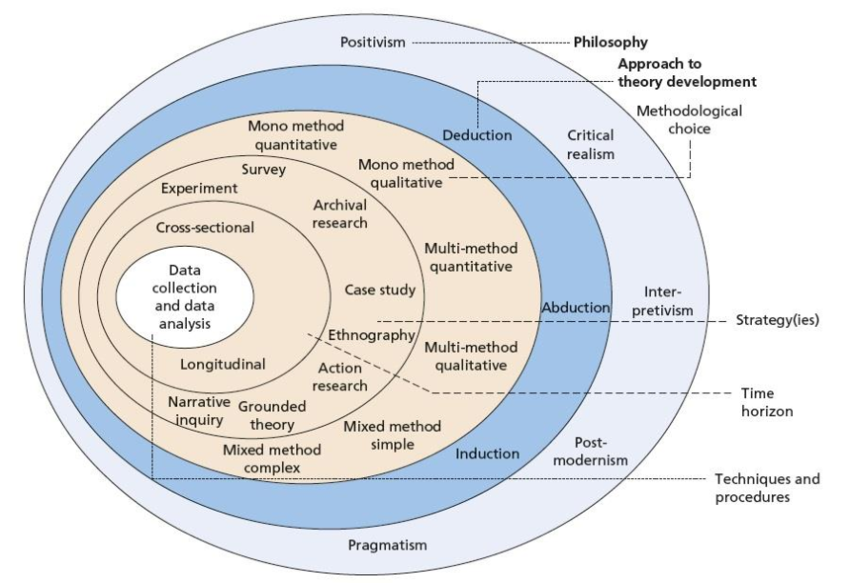
\includegraphics[width=.8\linewidth]{figures/Research-onion-4.png}
    \caption{The research onion (adopted from \cite{siti2020}). [for illustration purposes only, so remove from the EA].}
    \label{fig:onion}
\end{figure}

You may want to insert \texttt{Python} code snippets to show the design of your algorithm. We created a \texttt{Python} macro in the preamble that makes it easy to insert snippets of code. This environment takes two arguments \verb|\begin{python}(caption)(label)| where:
\begin{enumerate}
    \item \textit{caption} can be used to provide a description for this code listing
    \item \textit{label} can be used as an identifier to reference this listing in the text
\end{enumerate}

\noindent As an example, consider listing~\ref{lst:foo}.

\begin{python}{Important algorithm}{lst:foo}
def foo(x: int, y: float) -> str:
    z = x + y
    return "Hello " + z
\end{python}

\noindent There is also the option to write pseudo code in \LaTeX. See the following example in algorithm~\ref{alg:wfc}. 

\begin{algorithm}[H]
\caption{Simplified version of the Wave Function Collapse algorithm}\label{alg:wfc}
\hspace*{\algorithmicindent} \textbf{Input}: Sample image $img$;\\
\hspace*{\algorithmicindent} \textbf{Output}: Rendered output image
\begin{algorithmic}[1]
\Function{WFC}{$img$}
\State patterns := ExtractFromSample($img$);
\State ConstructIndex(patterns);
\State InitialiseGrid(patterns);
\Repeat 
    \State $p$ := Observe();
    \If{$p = null$}
        \State \textbf{break};
    \EndIf
    \State Collapse($p$);
    \State Propagate();
\Until{all variables are observed}
\State \Return ObservationsToOutput(); 
\EndFunction
\end{algorithmic}
\end{algorithm}

\noindent Often, you evaluate your artifacts quantitatively, elicit requirements from stakeholders, or may aggregate guidelines from the contemporary literature. In these cases, it can be useful to display these results in a table. See table~\ref{tab:example1},~\ref{tab:example2}, and~\ref{tab:example3} for various table examples. 

\def\arraystretch{1.5}%  1 is the default, change whatever you need
\begin{table}[H]
    \centering
    \caption{Confusion matrix for two classes.}
    \label{tab:example1}
    \vspace{-2mm}
    \begin{tabular}{|c|c|c|c|}
    \hline
        & \multicolumn{3}{c|}{\textit{Predicted class}} \\\hline
        \textit{True class} & \textbf{Positive} & \textbf{Negative} & \textit{Total} \\\hline
        \textbf{Positive} & $tp$: true positive & $fn$: false negative & $p$\\\hline
        \textbf{Negative} & $fp$: false positive & $tn$: true negative & $n$\\\hline
        \textit{Total} & $p'$ & $n'$ & $N$\\\hline
    \end{tabular}
\end{table}

\begin{table}[H]
    \centering
    \caption{Evaluation results of the selected hypothesis classes over 98 repetitions of training/testing splits for both the baseline as well as the difference datasets. Mean AUC and cross-entropy loss are reported. }\label{tab:example2}
    \vspace{-2mm}
    \makebox[\linewidth]{
        \begin{tabular}{l|cc|cc}
            \toprule
                \multicolumn{1}{c}{} & \multicolumn{2}{c}{\textbf{Baseline}} & \multicolumn{2}{c}{\textbf{Difference}} \\ 
            \cmidrule(rl){2-3} \cmidrule(rl){4-5}
                \textbf{Model} & \emph{AUC} & \emph{Cross-entropy} & \emph{AUC} & \emph{Cross-entropy} \\
            \midrule
                Random Forest & $0.605 \pm 0.010$ & $12.227 \pm 0.332$ & $0.609 \pm 0.012$ & $12.281 \pm 0.377$ \\
                XGBoost Classifier & $0.617 \pm 0.014$ & $12.474 \pm 0.456$ & $0.612 \pm 0.012$ & $12.314 \pm 0.394$ \\
                Support Vector Machine & $0.560 \pm 0.017$ & $15.220 \pm 0.631$ & $0.511 \pm 0.007$ & $14.453 \pm 0.242$ \\
                Multi-Layer Perceptron & $\bm{0.622 \pm 0.012}$ & $\bm{12.096 \pm 0.423}$ & $\bm{0.618 \pm 0.011}$ & $\bm{12.155 \pm 0.355}$ \\
            \bottomrule
        \end{tabular}
    }
\end{table}

\begin{table}[H]
    \centering
    \caption{Hyperparameter search space for the Random Forest classifier.}\label{tab:example3}
    \vspace{-2mm}
    \makebox[\linewidth]{
        \begin{tabularx}{\textwidth}
        % {lXr}
         {
            >{\raggedright\arraybackslash}p{.24\textwidth}
            >{\raggedright\arraybackslash}p{.4\textwidth}
            X
        }
            \toprule
                \textbf{Parameter} & \textbf{Description} & \textbf{Values} \\
            \midrule
                \texttt{n\_estimators} & Number of decision tree estimators. & $[50, 5000]$ with steps of 50.\\
                \texttt{min\_samples\_leaf} & Minimum number of instances required at a leaf node. & $[5, 50]$ with steps of 5.\\
                \texttt{max\_depth} & Maximum depth of the decision trees. & $[4, 24]$\\
                \texttt{criterion} & Function to measure quality of a split. & \texttt{'gini'} or \texttt{'entropy'}\\
                \texttt{max\_features} & For $d$ features, it is the $k<d$-features to consider when looking for the best split. & $\sqrt{d}$ or $\log_2(d)$, or fractions of $d$: 0.1, 0.3, 0.5, 0.7, 0.9. \\
                \texttt{bootstrap} & Whether bootstrap samples are used when building trees. & \texttt{True} or \texttt{False}\\
            \bottomrule
        \end{tabularx}
    }
\end{table}
\section{Discussion}

Maximum of 400 words.

The discussion describes a critical view (reflection) of the author(s) on the work delivered as a whole:
\begin{itemize}
    \item Which aspects have contributed positively to the results achieved and why?
    \item Which aspects have been limiting for the results achieved and why?
\end{itemize}

Aspects can be considered broadly here. For example, process choices (method),
design decisions (results) or other (whether or not externally determined) aspects that have influenced the results
\section{Conclusions}

Maximum of 400 words.
The conclusion describes the extent to which the original goal of the assignment has been met with the help of the achieved (factual, substantive)
results. In addition, any recommendations for follow-up work are described:
\begin{itemize}
    \item Which artefacts have/have not been realised?
    \item To what extent have any boundary conditions/requirements been met?
    \item To what extent can the results be used/used for the original
purpose?
    \item What recommendations are made on the basis of this, both towards practice and
any necessary follow-up research into previously carried out work?
\end{itemize}


\newpage
\printbibliography % this adds the bibliography to your document

\newpage
\appendix
\appendixpage

\input{appendix}


\end{document}
